%\documentclass[12pt,a4paper]{article}
%
%\usepackage{amsmath, amssymb}
%\usepackage[utf8]{inputenc}
%\usepackage[english]{babel}
%\usepackage{graphicx}
%\usepackage[margin=0.5in]{geometry}
%\usepackage{float}
%
%\graphicspath{{fig/}}
%
%
%\begin{document}
\subsection*{Level 1}
The model following part were derived by inverting each block of the DC motor model step by step and was verified by using outputs from the DC motor model as input for the inverse model. This should yield the same input for the DC motor model as output for the inverse model and it did. \\
\\
In order to design the trajectory planner values for $a_{max}$ and $v_{max}$ needed to be decided. $v_{max}$ was read from a velocity plot when the motor model was fed with 24 V. $a_{max}$ was calculated to a value around 600-700 but that value saturated the voltage from the model follower. $a_{max}$ was therefore tweaked into a value which never saturates the voltage. The values derived can be seen in the following table.
\begin{center}
	\begin{tabular}{| c | c |}
		\hline
		$a_{max}$ & 255 \\ \hline
		$v_{max}$ & 270 \\ 
		\hline
	\end{tabular}
\end{center}

The signal from the trajectory planner with Rs = 10 and Rs=100 can be seen in Figure \ref{fig:task2_pos}.

\begin{figure}[H]
	\begin{center}
	
		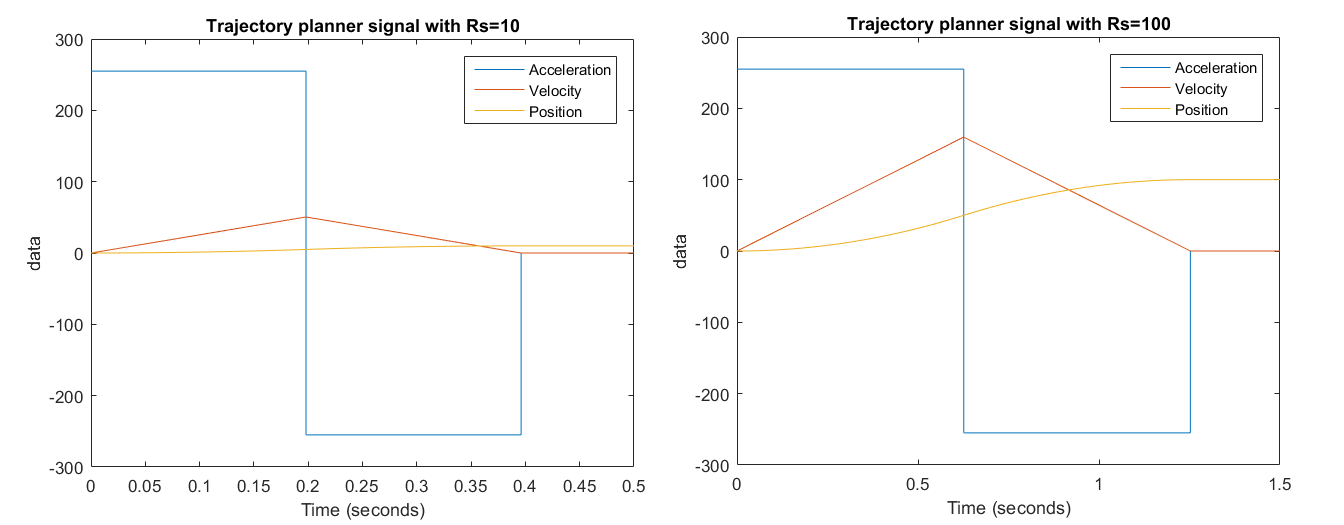
\includegraphics[width=\linewidth]{task1_traj_rs10.png}
		\caption{The trajectory planner with different Rs values}
		\label{fig:task2_pos}
	\end{center}
\end{figure}


%\end{document}